\documentclass{article}
\usepackage{amsmath}
\usepackage{amsthm}
\usepackage{biblatex}
\usepackage{graphicx}
\usepackage{hyperref}
\usepackage{cleveref}

\theoremstyle{plain}
\newtheorem{theorem}{Theorem}[section]
\newtheorem{corollary}{Corollary}[section]
\newtheorem{lemma}{Lemma}[section]
\newtheorem{proposition}{Proposition}[section]

\theoremstyle{definition}
\newtheorem{definition}{Definition}[section]
\newtheorem{example}{Example}

\theoremstyle{remark}
\newtheorem{remark}{Remark}[section]
\newtheorem{fact}[remark]{Fact}
\DeclareMathOperator{\aff}{aff}

\addbibresource{bibliography.bib}
\title{An example of how to use this plugin}
\author{Matthew Scott}
\begin{document}
\maketitle
\begin{abstract}
This is the abstract.
\end{abstract}
\section{Introduction}
\label{loc:body.introduction}
We \emph{have} \textbf{things} ``to" talk about. We can use macros: $\aff(T)$. Feel free to skip ahead to \autoref{loc:body.main_results}. This is the actual intro. We will show that \autoref{loc:theorem_1.statement} holds by using \autoref{loc:lemma_1.statement}, \autoref{loc:lemma_2.statement}, \autoref{loc:other_small_lemmas.first_other_lemma} and \autoref{loc:other_small_lemmas.second_other_lemma}. We state one here
\begin{lemma}

\label{loc:other_small_lemmas.second_other_lemma}
That the first lemma holds
\end{lemma}
\section{Literature review}
\label{loc:body.literature_review}
We cite \textcite{vershyninHighDimensionalProbabilityIntroduction2018} because it is a good book. It is by \cite[txt]{vershyninHighDimensionalProbabilityIntroduction2018}. Specifically, see \cite[Example 5.4]{vershyninHighDimensionalProbabilityIntroduction2018}. Other relevant sources are \cite{berkCoherenceParameterCharacterizing2022, berkModeladaptedFourierSampling2023}.
\section{Main results}
\label{loc:body.main_results}
Here is an equation that we can reference.
\begin{equation}
\label{eq:main}
1+1 = 2
\end{equation}
\begin{lemma}
We could say that
\begin{equation*}
1+1  = 2
\end{equation*}
as in \autoref{eq:main}, but we will not.
\begin{align}
1+1 & = 1+3-2 \label{eq:aligned_eq:1}\\
& = 2 \label{eq:aligned_eq:2}
\end{align}
Notice that \autoref{eq:aligned_eq:1} and \autoref{eq:aligned_eq:2} follows from arithmetic.
\end{lemma}
{#lem-explicit}
Since \autoref{lem:explicit} failed to help us, we employ the following result.
\begin{theorem}

\label{loc:theorem_1.statement}
Indeed, $1+1  =  2$.
\end{theorem}
See \hyperlink{loc:theorem_1.proof}{the proof}. To prove \autoref{loc:theorem_1.statement}, we need the following two results.
\begin{lemma}

\label{loc:lemma_1.statement}
The first fact is that $10-9 = 1$
\end{lemma}
We defer \hyperlink{loc:lemma_1.proof}{the proof} to the appendix.
\begin{lemma}

\label{loc:other_small_lemmas.first_other_lemma}
A first additional lemma
\begin{equation*}
1+1 = 2
\end{equation*}
\end{lemma}
We can reference: 
\begin{enumerate}
\item \autoref{loc:other_small_lemmas.first_other_lemma} and 
\item The other,\autoref{loc:other_small_lemmas.second_other_lemma}.
\end{enumerate}
% This will become a comment in latex.
\section{Proofs}
\label{loc:body.proofs}
We are ready to prove our main result.
\begin{proof}
[\hypertarget{loc:theorem_1.proof}Proof of \autoref{loc:theorem_1.statement}]For this we require another result.
\begin{proposition}

\label{loc:lemma_2.statement}
$1+4 = 5$
\end{proposition}
\begin{proof}
[\hypertarget{loc:lemma_2.proof}Proof of \autoref{loc:lemma_2.statement}]Left to the reader.
\end{proof}
and therefore we can finish the proof of \autoref{loc:theorem_1.statement}.
\end{proof}
\section{Numerics}
\label{loc:body.numerics}
Behold!
\begin{figure}[h]
\centering
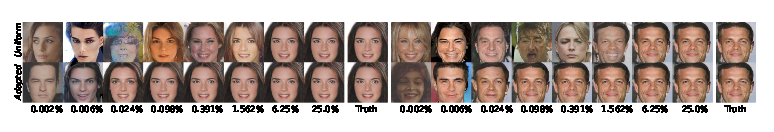
\includegraphics[width=0.5\textwidth]{Files/intro_comp_wlabel.pdf}
\caption{Notice that this is a great plot.\label{fig:intro_comp_wlabel.pdf}}
\end{figure}
We can reference the above \autoref{fig:intro_comp_wlabel.pdf}.
\printbibliography
\appendix
\section{Appendix}
\begin{proof}
[\hypertarget{loc:lemma_1.proof}Proof of \autoref{loc:lemma_1.statement}]Ask chatgpt.
\end{proof}
\end{document}
